%%%%%%%%%%%%%%%%%%%%%%%%%%%%%%%%%%%%%%%%%%%%%%%%%%%%%%%%%%%%%%%%
%                         My Template:                         %
%%%%%%%%%%%%%%%%%%%%%%%%%%%%%%%%%%%%%%%%%%%%%%%%%%%%%%%%%%%%%%%%

%Code(C++): \begin{lstlisting}
%Algorithm:
%\begin{breakablealgorithm}
%  \caption{?statement}
%  \begin{algorithmic}[?number]
%    \Require ?input
%    \Ensure ?output
%    \Procedure{Equal}{?parameters}
%      \State ?blabla
%    \EndProcedure
%  \end{algorithmic}
%\end{breakablealgorithm}

%Itemlisting: \begin{itemize} or \begin{enumerate}[label=(\alph*)]

%Math equation: \begin{align*}

%Table: \begin{tabular}{|c|c|c|}
%           blabla | blabla | blabla \\
%           ......
%Picture: \centerline{\includegraphics[scale=X]{FileName}

%%%%%%%%%%%%%%%%%%%%%%%%%%%%%%%%%%%%%%%%%%%%%%%%%%%%%%%%%%%%%%%%
%                         Title START!                         %
%%%%%%%%%%%%%%%%%%%%%%%%%%%%%%%%%%%%%%%%%%%%%%%%%%%%%%%%%%%%%%%%
\documentclass[11pt, a4paper, UTF8]{ctexart}

    %%%%%%%%%%%%%%%%%%%%%%%%%%%%%%%%%%%
% File: preamble.tex
%%%%%%%%%%%%%%%%%%%%%%%%%%%%%%%%%%%
\usepackage{geometry}
\geometry{left = 1cm, right = 1cm, top = 1.5cm, bottom = 1.5cm}

\ProvidesPackage{zhfontcfg}
\usepackage{fontspec,xunicode}
\usepackage{xeCJK}
\usepackage{CJKutf8}
\usepackage{enumerate}
\defaultfontfeatures{Mapping=tex-text}
\XeTeXlinebreaklocale "zh"
\XeTeXlinebreakskip = 0pt plus 1pt minus 0.1pt
% Set fonts commands
% \newcommand\fontnamehei{文泉驿正黑}
% \newcommand\fontnamesong{文鼎PL新宋}
% \newcommand\fontnamekai{AR PL UKai CN}
% \newcommand\fontnamemono{Bitstream Vera Sans Mono}
% \newcommand\fontnameroman{Bitstream Vera Serif}
% \newcommand{\song}{\fontnamesong}
% \newcommand{\hei}{\fontnamehei}
% \newfontinstance\KAI {\fontnamekai}
% \newcommand{\kai}{\fontnamekai}
% \newCJKfontfamily\kai{FandolKai-Regular.otf}
% \newCJKfontfamily\hei{FandolHei-Regular.otf}
% \newCJKfontfamily\song{FandolSong-Regular.otf}
% \newCJKfontfamily\fang{FandolFang-Regular.otf}
% \setCJKfamilyfont{song}[BoldFont=FandolSong-Bold.otf]{FandolSong-Regular.otf}
% \setCJKfamilyfont{hei}{FandolHei-Regular.otf}
% \setCJKfamilyfont{kai}{FandolKai-Regular.otf}
\newcommand{\song}{\CJKfamily{song}}
\newcommand{\hei}{\CJKfamily{hei}}
\newcommand{\kai}{\CJKfamily{kai}}
\newcommand{\fs}{\CJKfamily{fs}}
\newcommand{\tqs}{\textquotesingle}

\defaultfontfeatures{
    Path = /usr/local/texlive/2018/texmf-dist/fonts/opentype/public/fontawesome/ }
\usepackage{fontawesome}
\newcommand{\me}[2]{\author{{\bfseries 姓名:}\underline{#1}\hspace{2em}{\bfseries 学号:}\underline{#2}}}

% Always keep this.
\newcommand{\noplagiarism}{
    \begin{center}
        \fbox{\begin{tabular}{@{}c@{}}
            请独立完成作业,不得抄袭。\\
            若参考了其它资料,请给出引用。\\
            鼓励讨论,但需独立书写解题过程。
        \end{tabular}}
    \end{center}
}

% Each hw consists of three parts:
% (1) this homework
\newcommand{\beginthishw}{\part{作业\faTasks}}
% (2) corrections (Optional)
\newcommand{\begincorrection}{\part{订正\faRefresh}}
% (3) any feedback (Optional)
\newcommand{\beginfb}{\part{反馈\faShareSquareO}}

% For math
\usepackage{amsmath}
\usepackage{amsfonts}
\usepackage{amssymb}
\usepackage{graphicx}
\usepackage{listings}
\usepackage{xcolor}
\usepackage{clrscode3e}
\usepackage{enumitem}
\usepackage{tikz}
\usepackage{tabularx}
\usepackage{multirow}
\newcolumntype{Y}{>{\centering\arraybackslash}X}
\newcolumntype{P}{>{\centering\arraybackslash}p}
%bigger integrate symbol
\usepackage{exscale}
\usepackage{relsize}
\usepackage{textcomp}

% colors
\newcommand{\red}[1]{\textcolor{red}{#1}}
\newcommand{\blue}[1]{\textcolor{blue}{#1}}
\newcommand{\teal}[1]{\textcolor{teal}{#1}}

% algorithms
\usepackage[]{algorithm}
\usepackage[noend]{algpseudocode} % noend
\makeatletter
\newenvironment{breakablealgorithm}
  {% \begin{breakablealgorithm}
      \begin{center}
          \refstepcounter{algorithm}% New algorithm
          \hrule height.8pt depth0pt \kern2pt% \@fs@pre for \@fs@ruled 画线
          \renewcommand{\caption}[2][\relax]{% Make a new \caption
              {\raggedright\textbf{\ALG@name~\thealgorithm} ##2\par}%
          \ifx\relax##1\relax % #1 is \relax
          \addcontentsline{loa}{algorithm}{\protect\numberline{\thealgorithm}##2}%
          \else % #1 is not \relax
          \addcontentsline{loa}{algorithm}{\protect\numberline{\thealgorithm}##1}%
          \fi
          \kern2pt\hrule\kern2pt
          }
          }{% \end{breakablealgorithm}
              \kern2pt\hrule\relax% \@fs@post for \@fs@ruled 画线
  \end{center}
  }
\makeatother
\renewcommand{\algorithmicrequire}{\textbf{Input:}} % Use Input in the format of Algorithm
\renewcommand{\algorithmicensure}{\textbf{Output:}} % Use Output in the format of Algorithm
% See [Adjust the indentation whithin the algorithmicx-package when a line is broken](https://tex.stackexchange.com/a/68540/23098)
\newcommand{\algparbox}[1]{\parbox[t]{\dimexpr\linewidth-\algorithmicindent}{#1\strut}}
\newcommand{\hStatex}[0]{\vspace{5pt}}
\makeatletter
\newlength{\trianglerightwidth}
\settowidth{\trianglerightwidth}{$\triangleright$~}
\algnewcommand{\LineComment}[1]{\Statex \hskip\ALG@thistlm \(\triangleright\) #1}
\algnewcommand{\LineCommentCont}[1]{\Statex \hskip\ALG@thistlm%
  \parbox[t]{\dimexpr\linewidth-\ALG@thistlm}{\hangindent=\trianglerightwidth \hangafter=1 \strut$\triangleright$ #1\strut}}
\makeatother


% Define theorem-like environments
\usepackage[amsmath, thmmarks, framed]{ntheorem}
\usepackage{framed}

\theoremheaderfont{\kai\bfseries}
\theoremstyle{break}
\theorembodyfont{\song}
% \theorembodyfont{\kai}
\theoremseparator{\vspace{1mm}}
\renewcommand*\FrameCommand{{\color{gray}\vrule width 3pt \hspace{10pt}}}
\newframedtheorem{problem}{\faCheckSquareO \ Problem}

\theorempostwork{\hrule}
\newtheorem*{solution}{\faEdit \ Solution}
\newtheorem*{revision}{\faEdit \ Revision}

\theoremstyle{plain}
\newtheorem*{cause}{\faCoffee \ Cause}
\newtheorem*{remark}{\faCommentingO \ Remark}

\theoremstyle{break}
\theoremsymbol{\ensuremath{\Box}}
\newtheorem*{proof}{\faEdit \ Proof}

\renewcommand\figurename{Figure}
\renewcommand\tablename{Table}

%enumeration
\setenumerate[1]{
    itemsep=0pt,
partopsep=0pt,
parsep=\parskip,
topsep=0pt,
leftmargin=20pt
}
\setitemize[1]{
    itemsep=0pt,
partopsep=0pt,
parsep=\parskip,
topsep=0pt,
leftmargin=20pt
}
\setdescription{
    itemsep=0pt,
partopsep=0pt,
parsep=\parskip,
topsep=0pt,
leftmargin=20pt
}
\lstset{
    language={[ISO]C++},
numbers=left,
numberstyle= \tiny,
commentstyle=\color{red!50!green!50!blue!50},
rulesepcolor=\color{red!20!green!20!blue!20},
keywordstyle=\color{blue!90}\bfseries,
showstringspaces=false,
stringstyle=\ttfamily,
}

% For figures
% for fig with caption: #1: width/size; #2: fig file; #3: fig caption
\newcommand{\fig}[3]{
    \centerline{\includegraphics[scale=#1]{#2}}
    \centerline{#3}
}

% for fig without caption: #1: width/size; #2: fig file
\newcommand{\fignc}[2]{
    \centerline{\includegraphics[scale=#1]{#2}}
}



    \title{Homework 2}
    \me{毕秋宇}{171860624}
    \date{\today}

    \begin{document}
    \maketitle
    % \noplagiarism

    %%%%%%%%%%%%%%%%%%%%%%%%%%%%%%%%%%%%%%%%%%%%%%%%%%%%%%%%%%%%%%%%
    %                       Homework START!                        %
    %%%%%%%%%%%%%%%%%%%%%%%%%%%%%%%%%%%%%%%%%%%%%%%%%%%%%%%%%%%%%%%%
    \beginthishw
    %%%%%%%%%%%%%%%%%%%%
    \begin{problem}[Multi-Label Logistic Regression]
        In multi-label problem, each instance $x$ has a label set $y = \{y_1 , y_2 ,\cdots, y_l \}$ and each label $y_i \in \{0, 1\}$. Assume the post probability $p(y|x)$ follows the conditional independence:
        \[p(y|x)=\prod_{i=1}^{l}p(y_{i}|x)\]
        Please use the logistic regression method to handle the following questions.
        \begin{enumerate}
            \item $[15pts]$ Please give the ’log-likelihood’ function of your logistic regression model;
            \item $[10pts]$ Please calculate the gradient of your ’log-likelihood’ function.
        \end{enumerate}
    \end{problem}

    %\begin{remark}

    %\end{remark}

    \begin{solution}
        Because the post probability $p(y|x)$ follows the conditional indenendence, so every label is independent. We can make $z_{i}=w_{i}^{T}x+b_{i}$, that is
        \[\left(
        \begin{matrix}
            z_{1}\\
            \vdots\\
            z_{m}
        \end{matrix}
        \right)=
        \left(
        \begin{matrix}
            w_{1}^{T}\\
            \vdots\\
            w_{m}^{T}
        \end{matrix}
        \right)\times
        \left(
        \begin{matrix}
            x_{1}\\
            \vdots\\
            x_{n}
        \end{matrix}
        \right)+
        \left(
        \begin{matrix}
            b_{1}\\
            \vdots\\
            b_{m}
        \end{matrix}
        \right)=
        \left(
        \begin{matrix}
            w_{11} & \cdots & w_{1n}\\
            \vdots & \cdots & \vdots\\
            w_{m1} & \cdots & w_{mn}
        \end{matrix}
        \right)\times
        \left(
        \begin{matrix}
            x_{1}\\
            \vdots\\
            x_{n}
        \end{matrix}
        \right)+
        \left(
        \begin{matrix}
            b_{1}\\
            \vdots\\
            b_{m}
        \end{matrix}
        \right)
        \]
        \begin{enumerate}
            \item[(1)] The likelihood function of the logistic regression model is:
                \[L(x_{1},x_{2},\cdots,x_{n})=\prod_{j=1}^{n}p(y|x_{j})=\prod_{j=1}^{n}\prod_{i=1}^{l}p(y_{i}|x_{j})\]
                So the log-likelihood function of it is:
                \[\log{L(x_{1},x_{2},\cdots,x_{n})}=\log{\prod_{j=1}^{n}p(y|x_{j})}=\log{\prod_{j=1}^{n}\prod_{i=1}^{l}p(y_{i}|x_{j})}=\sum_{j=1}^{n}\sum_{i=1}^{l}\log{p(y_{i}|x_{j})}\]
            \item[(2)]
                \[\nabla \log L(x_{1},\cdots,x_{n})=[\frac{\partial{\sum_{i=1}^{l}\log p(y_{i}|x_{1})}}{\partial{x_{1}}},\cdots,\frac{\partial{\sum_{i=1}^{l}\log p(y_{i}|x_{n})}}{\partial{x_{n}}}]^{T}\]
        \end{enumerate}
    \end{solution}
    %%%%%%%%%%%%%%%%%%%%%
    \begin{problem}[Linear Discriminant Analysis]
        Suppose we transform the original $\mathbf{X}$ to $\mathbf{\hat{Y}}$ via linear regression . In detail, let
        \[\mathbf{\hat{Y}} = \mathbf{X}(\mathbf{X^{T}}\mathbf{X^{-1}})^{-1}\mathbf{X^{T}}\mathbf{Y} = \mathbf{X}\mathbf{\hat{B}},\]
        where $\mathbf{X}$ and $\mathbf{Y}$ are the feature and label matrix, respectively. Similarly for any input $\mathbf{x}$, we get a transformed vector $\mathbf{\hat{y}}= \mathbf{\hat{B}^{T}}\mathbf{x}$. Show that $LDA$ using $\mathbf{\hat{Y}}$ is identical to $LDA$ in the original space.
    \end{problem}

    %\begin{remark}

    %\end{remark}

    \begin{solution}
        Because we have that $\mathbf{\hat{y}}= \mathbf{\hat{B}^{T}}\mathbf{x}$, so $\hat{\mu}_{k}^{\hat{y}}=\hat{B}^{T}\hat{\mu}_{k}^{x}$ and $\hat{\mu}_{l}^{\hat{y}}=\hat{B}^{T}\hat{\mu}_{l}^{x}$.\\
        That is to say,
        \[\log{\frac{\Pr(G=k|\hat{Y}=\hat{y})}{\Pr(G=l|\hat{Y}=\hat{y})}}=\log{\frac{f_{k}(\hat{y})}{f_{l}(\hat{y})}}+\log{\frac{\pi_{k}}{\pi_{l}}}=\log{\frac{\pi_{k}}{\pi_{l}}}-\frac{1}{2}(\hat{\mu}_{k}^{\hat{y}}+\hat{\mu}_{l}^{\hat{y}})^{T}\Sigma^{-1}_{y}(\hat{\mu}_{k}^{\hat{y}}-\hat{\mu}_{l}^{\hat{y}})+\hat{y}^{T}\Sigma^{-1}_{y}(\hat{\mu}_{k}^{\hat{y}}-\hat{\mu}_{l}^{\hat{y}})\]
        \[=\log{\frac{\pi_{k}}{\pi_{l}}}-\frac{1}{2}(\hat{\mu}_{k}^{\hat{x}}+\hat{\mu}_{l}^{\hat{x}})^{T}\hat{B}\Sigma^{-1}_{y}\hat{B}^{T}(\hat{\mu}_{k}^{\hat{x}}-\hat{\mu}_{l}^{\hat{x}})+\hat{x}^{T}\hat{B}\Sigma^{-1}_{y}\hat{B}^{T}(\hat{\mu}_{k}^{\hat{x}}-\hat{\mu}_{l}^{\hat{x}})\]
        According to the equation in ESL 4.9.\\
        So We need to prove that
        \[\hat{B}\Sigma^{-1}_{y}\hat{B}^{T}=\Sigma^{-1}_{x}\]
        We also know
        \[\Sigma_{y}=\frac{\sum_{k=1}^{N}\sum_{g_{i}=k}(\hat{y}_{i}-\hat{\mu}_{k}^{\hat{y}})(\hat{y}_{i}-\hat{\mu}_{k}^{\hat{y}})^{T}}{N-K}=\frac{\sum_{k=1}^{N}\sum_{g_{i}=k}\hat{B}^{T}(\hat{x}_{i}-\hat{\mu}_{k}^{\hat{x}})(\hat{x}_{i}-\hat{\mu}_{k}^{\hat{x}})^{T}\hat{B}}{N-K}=\hat{B}^{T}\Sigma_{x}\hat{B}.\]
        \[\Rightarrow\hat{B}\Sigma^{-1}_{y}\hat{B}^{T}=\hat{B}(\hat{B}^{T}\Sigma_{x}\hat{B})^{-1}\hat{B}^{T}=\hat{B}\hat{B}^{-1}\Sigma_{x}^{-1}(\hat{B}^{T})^{-1}\hat{B}^{T}=\Sigma^{-1}_{x}\]
        So far, we have proved that $LDA$ using $\hat{Y}$ is identical to $LDA$ in the original space.
    \end{solution}
    %%%%%%%%%%%%%%%%%%%%%
    \begin{problem}[Logistic Regression from scratch]
        Implementing algorithms is a good way of understanding how they work in-depth. In case that you are not familiar with the pipeline of building a machine learning model, this article can be an example.\\
        In this experiment, you are asked to build a classification model on one of UCI data sets, Letter Recognition Data Set.\\
        In particular, the objective is to identify each of a large number of black-and-white.\\
        rectangular pixel displays as one of the 26 capital letters in the English alphabet. The detailed statistics of this data set is listed in Table. The data set was then randomly split into train set and test set with proportion $7:3$. Also, letters from `A' to `Z' are mapped to digits `1' to `26' respectively as represented in the last column of the provided data set.\\
        \begin{Table}
            \centering
            \vspace{2mm}
            % \caption{Statistics of the data set.}
            % \label{tab:dataset}
            \begin{tabular}{|c|c|c|}
                \hline
                Property & Value & Description\\
                \hline
                Number of Instances & 20,000 & Rows of the data set\\
                \hline
                Number of Features & 17 & Columns of the data set\\
                \hline
                Number of classes & 26 & Dimension of the target attribute \\
                \hline
            \end{tabular}
        \end{Table}

        In order to build machine learning models, you are supposed to implement Logistic Regression (LR) algorithm which is commonly used in classification tasks. Specifically, in this experiment, you have to adapt the traditional binary class LR method to tackle the multi-class learning problem.
        \begin{enumerate}
            \item[(1)] [\textbf{5pts}] You are encouraged to implement the code using \emph{Python3} or \emph{Matlab}, implementations in any other programming language will not be judged. Please name the source file (which contains the main function) as \emph{LR\underline{\hspace{0.5em}}main.py} (for python3) or \emph{LR\underline{\hspace{0.5em}}main.m} (for matlab). Finally, your code needs to print the testing performance on the provided test set once executed.

            \item[(2)] [\textbf{30pts}] Functions required to implement:
                \begin{itemize}
                    \item Implement LR algorithm using gradient descent or Newton's method.
                    \item Incorporate One-vs-Rest (OvR) strategy to tackle multi-class classification problem.
                \end{itemize}
            \item[(3)] [\textbf{20pts}] Explain implementing details in your submitted report (source code should not be included in your report), including optimization details and hyper-parameter settings, etc. Also, testing performance with respect to Accuracy, Precision, Recall, and $F_1$ score should be reported following the form of Table 2.
        \end{enumerate}

        \begin{Table}
            \centering
            % \caption{Performance of your implementation on test set.}
            \vspace{2mm}
            \label{tab:my_label}
            \begin{tabular}{|c|c|}
                \hline
                Performance Metric & Value (\%) \\
                \hline
                accuracy & 00.00 \\
                \hline
                micro Precision  & 00.00\\
                \hline
                micro Recall & 00.00\\
                \hline
                micro $F_1$ & 00.00\\
                \hline
                macro Precision  & 00.00\\
                \hline
                macro Recall & 00.00\\
                \hline
                macro $F_1$ & 00.00\\
                \hline
            \end{tabular}
        \end{Table}
        \textbf{NOTE:} Any off-the-shelf implementations of LR or optimization methods are \textbf{NOT ALLOWED} to use. When submitting your code and report, all files should be placed in the same directory (without any sub-directory).
    \end{problem}

    %\begin{remark}

    %\end{remark}

    \begin{solution}
        \

        Introduction : While implementing Logistic Regression, I use matrix multiplication instead of training every case to save the running time and guarantee the large number of epoch. In terms of chosing the hyper-parameter $\alpha$, which is normally called gradient in Maths, method of bisection is useful. I checked the gradient from $1$ to $1^{-7}$, and used the function $\alpha=\frac{0.01+\frac{0.01}{1+i}}{m}$ of epoch $i$ instead of just choosing a constant in order for a faster convergence. Finally, I implement the Logistic Regression with $100000$ epoch and the preformance is as follows
        \begin{figure}[H]
            \centering
            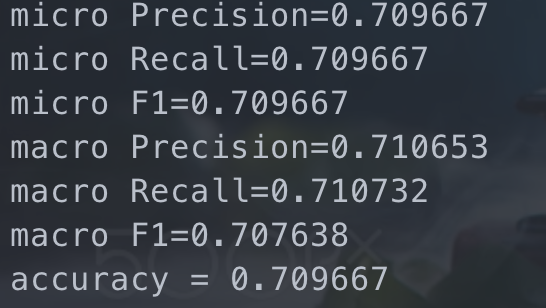
\includegraphics[width=0.5\linewidth]{1.png}
            \caption{Performance}
            \label{fig:mcmthesis-logo}
        \end{figure}

        Difficulties that I met : When writing the vote function, I create an array $[\ ]$ and assign it with prediction by parameters $1\sim 26$, then use function $index(max(array))+1$ to get the index of largest probability. However, the assignment will replace the original value, so $index(max(array))+1$ will always return $1$. After I using a loop to get the maximum of probability and the index of it, the problem is fixed.

    \end{solution}
    %%%%%%%%%%%%%%%%%%%%%
    % \begin{problem}[TC 32.3-1]
    % \end{problem}

    %\begin{remark}

    %\end{remark}

    % \begin{solution}
    %
    % \end{solution}
    %%%%%%%%%%%%%%%%%%%%%
    % \begin{problem}[TC 32.3-3]
    % \end{problem}

    %\begin{remark}

    %\end{remark}

    % \begin{solution}
    %
    % \end{solution}
    %%%%%%%%%%%%%%%%%%%%
    %\newpage
    %%%%%%%%%%%%%%%%%%%%


    %%%%%%%%%%%%%%%%%%%%%%%%%%%%%%%%%%%%%%%%%%%%%%%%%%%%%%%%%%%%%%%%
    %                      Correction START!                       %
    %%%%%%%%%%%%%%%%%%%%%%%%%%%%%%%%%%%%%%%%%%%%%%%%%%%%%%%%%%%%%%%%
\begincorrection
%%%%%%%%%%%%%%%%%%%%
%\begin{problem}[]

%\end{problem}

%\begin{cause}
%
%\end{cause}

%\begin{revision}

%\end{revision}
%%%%%%%%%%%%%%%%%%%%
%\newpage
%%%%%%%%%%%%%%%%%%%%


%%%%%%%%%%%%%%%%%%%%%%%%%%%%%%%%%%%%%%%%%%%%%%%%%%%%%%%%%%%%%%%%
%                       Feedback START!                        %
%%%%%%%%%%%%%%%%%%%%%%%%%%%%%%%%%%%%%%%%%%%%%%%%%%%%%%%%%%%%%%%%
\beginfb
%\begin{itemize}
%
%\end{itemize}


%%%%%%%%%%%%%%%%%%%%%%%%%%%%%%%%%%%%%%%%%%%%%%%%%%%%%%%%%%%%%%%%
%                        Homework END!                         %
%%%%%%%%%%%%%%%%%%%%%%%%%%%%%%%%%%%%%%%%%%%%%%%%%%%%%%%%%%%%%%%%
\end{document}

